
%\pdfbookmark[1]{Anexo}{Anexo}
%************************************************
\chapter{Identity Mixer protocol}\label{ch:idemix} 
%************************************************

En este anexo incluimos por completitud las pruebas de conocimiento cero no interactivas utilizadas durante la emisión de un certificado de Identity Mixer (\autoref{idemix:cert}).


\begin{figure}[bth]
	\begin{center}
		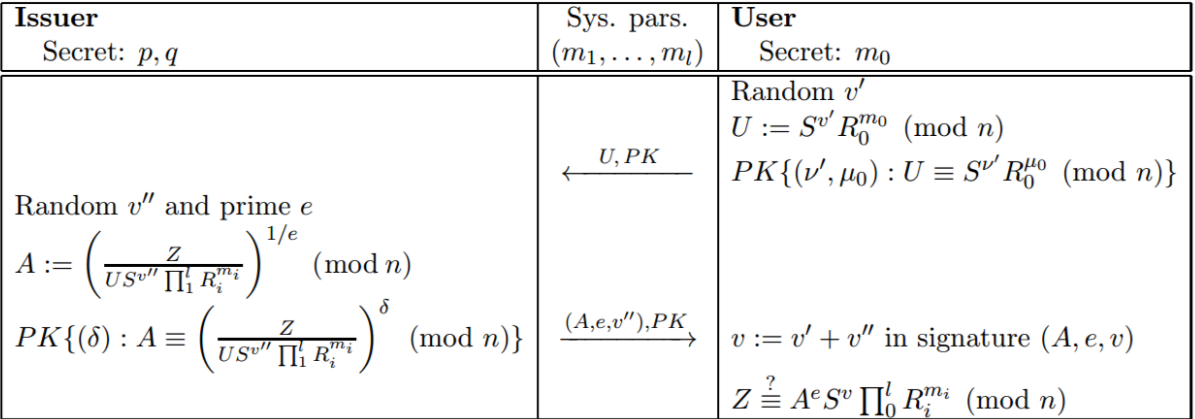
\includegraphics[width=0.8\linewidth]{gfx/issuanceIdemix}
	\end{center}
	\caption{Idemix: firma de credenciales simplificada.}
	\label{fig:issuanceIdemix}
\end{figure}

\hfil


La prueba de conocimiento $P_1$ indica que conocemos un $v'$, primera parte del $v$ final de la firma CL, y un $m_0$, nuestra clave secreta, tales que $U$ se representa como $(v', m_0)$ en la \textit{base} $(S,R_0)$. Utilizando la heurística de Fiat-Shamir, en vez de pedir varios retos al Emisor para conseguir robustez, utilizamos una función de hash junto a un reto $n_1$ del emisor, llamado en inglés \textit{nonce}. La prueba que se envía consiste en una tupla con el reto obtenido por el hash, y las respuestas a dicho reto.

\begin{algorithm}[$KP\{(v',m_0) : U \equiv S^{v'}R_0^{m_0} \, mod \, n \}(n_1)$]
	\hfil
	
	\begin{enumerate}
		\item Elegir $\tilde{m}_0$ y $\tilde{v}'$ aleatorios.
		\item Calcular $\tilde{U} = S^{\tilde{v}'}\cdot R_0^{\tilde{m}_0} \, mod \, n$.
		\item Reto por heurística Fiat-Shamir: $c = H(U||\tilde{U}||n_1)$.
		\item Respuestas al \textit{reto}: $\hat{v}' = \tilde{v}' + c v'$, $\hat{m}_0 = \tilde{m}_0 + c m_0$.
		\item $P_1 := (c, \hat{v}', \hat{m}_0)$.
	\end{enumerate}
	
\end{algorithm}

\hfil

Para verificar la prueba anterior, por la heurística de Fiat-Shamir (\ref{fiat-shamir-heur}), debemos \textit{recuperar} el valor de $U$ calculado por el Usuario, y comparar los hashes generados.

\begin{algorithm}[Verificar $P_1 := (c, \hat{v}', \hat{m}_0)(n_1)$]
	\hfil
	
	\begin{enumerate}
		\item Calcular $\hat{U} = U^{-c}\cdot S^{\hat{v}'} R_0^{\hat{m}_0} \, mod \, n$.
		\item Aceptar si $c = H(U||\hat{U}||n_1)$.
	\end{enumerate}
	
\end{algorithm}

\hfil


En la prueba de conocimiento $P_2$ del Emisor, demostramos que conocemos la inversa del $e$ de la firma CL, pero sin desvelar su valor, que solo el Emisor, conocedor de $p$ y $q$, puede calcular.

\begin{algorithm}[$KP\{(e^{-1}) : A \equiv \left( \frac{Z}{U\cdot S^{v''}\cdot \prod_{i=1}^{l} R_i^{m_i}} \right)^{e^{-1}} \, mod \, n \}(n_2)$]
	\hfil
	
	Llamemos $Q:=\frac{Z}{U\cdot S^{v''}\cdot \prod_{i=1}^{l} R_i^{m_i}}$.
	\begin{enumerate}
		\item Elegir $r$ aleatorio.
		\item Calcular $\tilde{A} = Q^r \, mod \, n$.
		\item Calcular el reto por Fiat-Shamir $c' = H(Q||A||n_2||\tilde{A})$.
		\item Calcular la respuesta $s_e = r-c'e^{-1}$.
		\item $P_2 := (c', s_e)$.
	\end{enumerate}
	
\end{algorithm}

\hfil

Como antes, para verificar la prueba, \textit{recuperamos} el valor $\tilde{A}$ y comparamos los hashes.

\begin{algorithm}[Verificar $P_2 := (c', s_e)(n_2)$]
	\hfil
	
	\begin{enumerate}
		\item Calcular $\hat{A} = A^{c'+s_e\cdot e} \equiv A^{c'}Q^{s_e} \, mod \, n$.
		\item Aceptar si $c' = H(Q||A||n_2||\hat{A})$.
	\end{enumerate}
	
\end{algorithm}
